The Gannt chart below describes the proposed timeline for the project. All items
within the Gannt chart are colour coded as follows; green represents
documentation - i.e. work on the final report, red represents background
research - i.e. background research required for understanding the topic, blue
represents testing - i.e. simulation testing, orange represents end of week
reviews, during which time the goals of the past week and following week will be
assessed.

\begin{figure}[H]
	\centering
	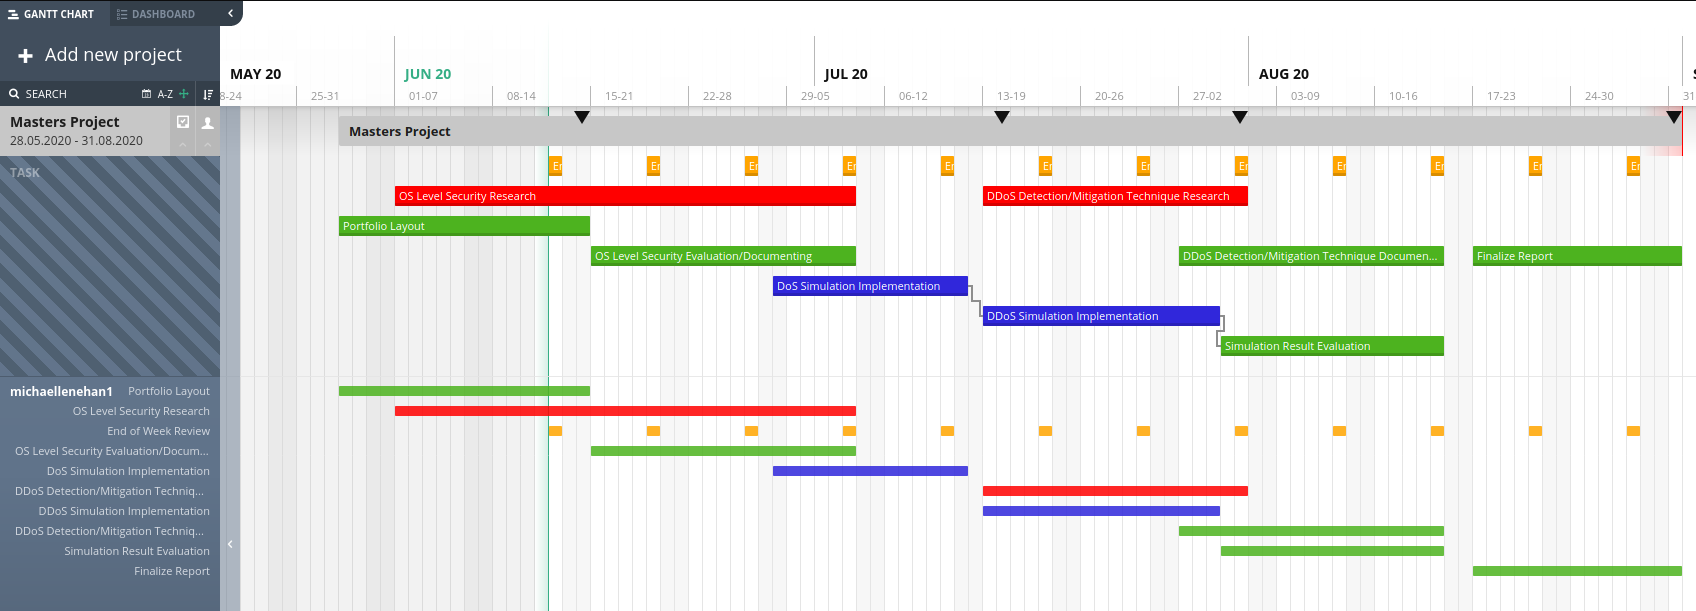
\includegraphics[width=\textwidth]{images/GanntChart}
	\caption{Project Gannt Chart}
	\label{fig:images-GanntChart}
\end{figure}

This project plan can be viewed at the following link:
\url{https://app.agantty.com/#/sharing/d595b7c64d314f5788834d0ed8614ccc/de}

Not included in this design plan are working hours, which, for the duration of
the project, will be 8 a.m. to 5 p.m Monday to Friday. All project work must be completed outside
of these times.
